% This LaTeX was auto-generated from an M-file by MATLAB.
% To make changes, update the M-file and republish this document.

\documentclass[12pt]{article}
\usepackage{natbib}
\usepackage[french]{babel}
\usepackage[utf8x]{inputenc}
\usepackage{lipsum}
\usepackage{amsmath}

\usepackage{graphicx}
\usepackage[final]{pdfpages}
\usepackage[T1]{fontenc}
%\usepackage[colorinlistoftodos]{todonotes}
\usepackage{xcolor}
\usepackage[nottoc,numbib]{tocbibind}% Para que la bibliografia salga en el table of contents
\colorlet{Mycolor1}{green!10!orange!90!}
\usepackage{subfigure}
\usepackage{plantuml}
\sloppy
\definecolor{lightgray}{gray}{0.5}
\setlength{\parindent}{0pt}
\setlength{\parskip}{1em}

\bibliographystyle{abbrv}

\begin{document}
\title{Rapport stage ASTC}
\author{CHIRINO CAICEDO Melet}
\begin{titlepage}

\newcommand{\HRule}{\rule{\linewidth}{0.5mm}} % Defines a new command for the horizontal lines, change thickness here

\center % Center everything on the page
 
%----------------------------------------------------------------------------------------
%	HEADING SECTIONS
%----------------------------------------------------------------------------------------

\textsc{\LARGE Université Toulouse III}\\[0.5cm] % Name of your university/college
\textsc{\Large Paul Sabatier}\\[1.0cm] % Major heading such as course name
\textsc{\large Rapport du stage 2021/2022}\\[0.5cm] % Minor heading such as course title

%----------------------------------------------------------------------------------------
%	TITLE SECTION
%----------------------------------------------------------------------------------------

\HRule \\[0.4cm]
{ \huge \bfseries Integration d'un logiciel embarqu\'e AUTOSAR en simulation}\\[0.4cm] % Title of your document
\HRule \\[1.5cm]
 
%----------------------------------------------------------------------------------------
%	AUTHOR SECTION
%----------------------------------------------------------------------------------------

\begin{minipage}{0.4\textwidth}
\begin{flushleft} \large
\markboth{Pojet en \LaTeX}
\emph{Auteurs:}\\
\textsc{CHIRINO} Melet \\ % Your name
%\textsc{RIBEIRO} Bruno % Your name
\end{flushleft}
\end{minipage}
~
\begin{minipage}{0.5\textwidth}
\begin{flushright} \large
\emph{Tuteur:} \\
\textsc{BROUEILH} Nicolas  % Supervisor's Name
\textsc{RIVI\`ERE} Nicolas  % Supervisor's Name
\end{flushright}
\end{minipage}\\[2cm]

% If you don't want a supervisor, uncomment the two lines below and remove the section above
%\Large \emph{Author:}\\
%John \textsc{Smith}\\[3cm] % Your name

%----------------------------------------------------------------------------------------
%	DATE SECTION
%----------------------------------------------------------------------------------------

{\large \today}\\[2cm] % Date, change the \today to a set date if you want to be precise

%----------------------------------------------------------------------------------------
%	LOGO SECTION
%----------------------------------------------------------------------------------------


\includegraphics[width=6in]{img/Logo_UT3.jpg}\\[2cm] % Include a department/university logo - this will require the graphicx package
 
%----------------------------------------------------------------------------------------

\vfill % Fill the rest of the page with whitespace

\end{titlepage}

%\{Contents}
\tableofcontents

\newpage

%-------------------------- * Introduccion * --------------------------------

\section{Introduction}
\section{Introduction}

\subsection{Description de la societ\'e}
Australian Semiconductor Technology Company (ASTC) est un fournisseur mondial des solutions logicielles et matériels pour les systèmes embarqués. Cette soci\'et\'e propose des services de conception, validation et vérification des systèmes sur puces et les circuits intégrés. Elle a développé son outil VLAB, qui fournit des solutions innovantes, pour la simulation des logiciels embarqués sur les plateformes Hardware virtuelles. La société a son siège à Adélaïde en Australie, elle possède des bureaux et des centres de R\&D à Toulouse, Tokyo, Illinois, Austin, et Texas. 

ASTC Desing partners a été créée \`a toulouse par Nicolas Broueilh et Eric Faure en 2014. Cette partie est plus focalis\'e en la conception de logiciel embarqu\'e, sourtout la virtualisation de hardware avec VLAB Works. Le produit le plus develop\'e est la toolbox \textit{AURIX} qui est capable de virtualiser la famille \textit{aurix} de \textit{Infineon Technologies AG}. Dans la figure \ref{fig:vlab-presentation} on peut voir un exemple de vlab.

VLAB utilise python2 pour accéder a tous les éléments de hardware virtuel et évènements de la simulation comme les ports du microcontroleur, registres, connections entre mod\`eles, temps de simulation, points d'arrête, etc. Pour les modèles de simulation il est utilis\'e C++ avec la librairie SystemC. Il y existe une API de SystemC pour python2 en raison de développer des mod\`eles plus rapidement mais moins performantes que celles en SystemC. Toutes les mod\`eles doivent \^etre compil\'es avant de d\'emarrer la simulation.

%Para programar en vlab es necesario usar python2 y con este podemos acceder a todos los elementos de la simulacion. Para los modelos es necesario hacerlo usando C++ y SystemC. Hay una API de SystemC para python lo cual permite hacer pequenhos modelos mas rapido pero eso tendra un impacto en la velocidad de la simulacion si no son compilados. Para los modelos que necesitan mas performance es mejor usar SystemC.

%Aqui empiezo hablando de que es astc, que es una empresa internacional que hace herramientas de simulacion de microcontroladores. Explico un poco que es vlab, un par de capturas de pantalla con la que se muestre sus caracteristicas funcionales y zas, juera. 

%Finalmente digo que mi stage se trata de modelizar un gateway ya existente con la herramienta de simulacion.

\begin{figure}[!htb]
    \centering
        \subfigure[Vlab Logo]{
\includegraphics [width=2.5in]{img/VLAB_Works.png}}
        \subfigure[Vlab en marche]{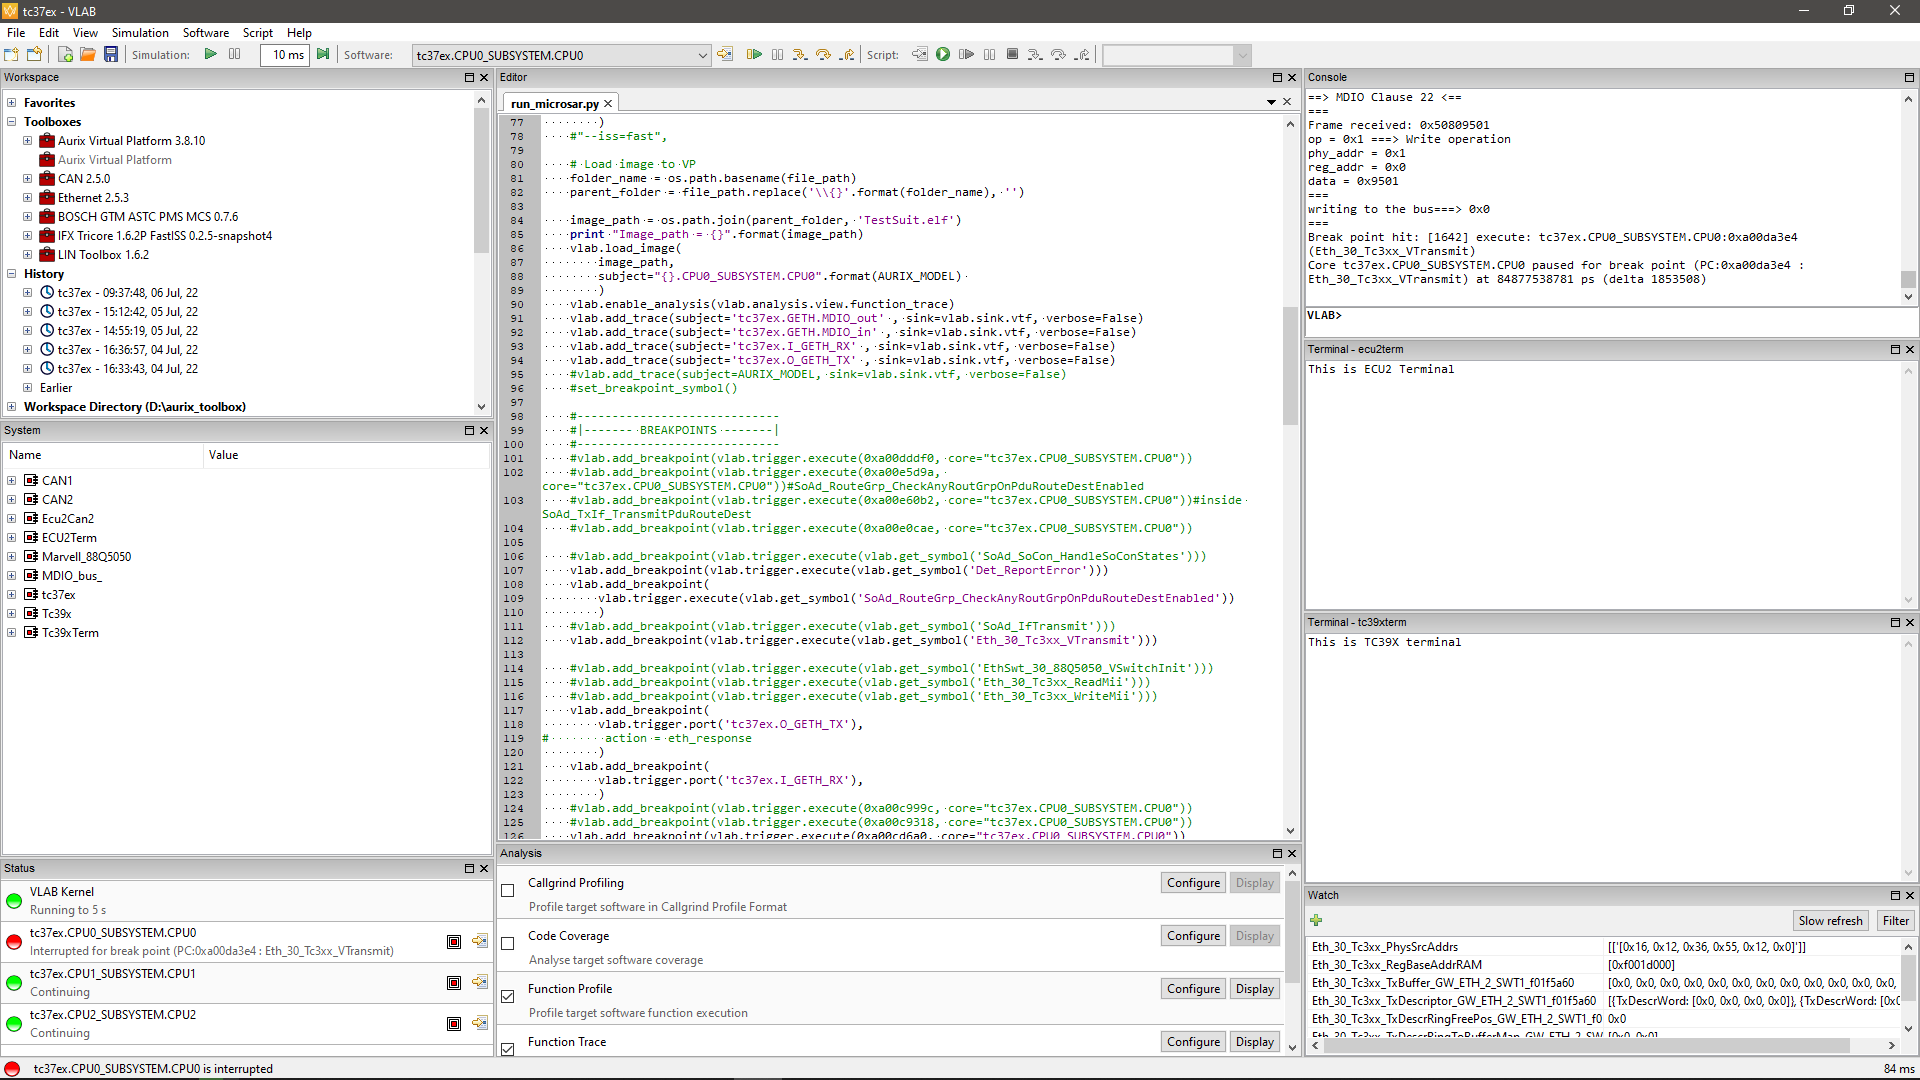
\includegraphics [width=5in]{img/vlab.png}}
    \caption{Vlab works}
    \label{fig:vlab-presentation}
\end{figure}

%\subsection{Virtualizacion y sus ventajas}


%-------------------------- * Descripcion * --------------------------------

\section{Descripcion del stage}
Ahora si explico bien que es el gateway, para que sirve, como se usa en la vida real y todo eso. Ademas debo decir que el gateway viene con su propio RTOS basado en autosar y que ellos quieren hacer una demo funcional de este gatway para mostrarle a los clientes mas adelante. El gateway viene con un OS ya predefinido para ese microcon pero no arranca porque inicialmente no esta conectado a nada.
%-------------------------- * Objetivos * --------------------------------

\section{Objectifs}
Mis objetivos... Debo preguntarle a Nico por mis objetivos precisos pero yo diria 
\begin{itemize}
    \item cargar microsar sobre un tc37x simulado y hacer que arranque
    \item Imitar las funcionalidades de canoe
    \item Hacer una UI (en pygame papu, eso me va a quedar para toda la vida)
\end{itemize}

\section{Conception}
Aqui vas a poner un pocoton de diagramas UML que expliquen lo que hiciste y describan los problemas que tuviste a la hora de poner en marcha todo

%-------------------------- * Seccion de resultados * --------------------------------

\section{Resultats}

Los resultados son prometedores despues de 3 semanas.

\subsection{Demarrage microsar}
Microsar al comienzo no queria arrancar porque el sistema simulado no soporta el BUS FlexRay tonces me toco "hackear" la tarjeta para que el sistema operativo viera que si lo soporta (incluso cuando no). Luego me toco hacer unas conexiones en el bus can y en el ASCLIN. 



%-------------------

%\begin{figure}[!htb]
%\centering
%\includegraphics[width=0.2\textwidth]{images/ubication-sipi.png}
%\caption{Location du village Sipí \cite{sipi:ubicacion}}
%\label{img:sipi:ubicacion}
%\end{figure}

% Plantilla para colocar muchas imagenes con un multiplot
%\begin{figure}[!htb]
%\centering
%\subfigure[Photo trouv\'e sur Facebook]{\includegraphics %[height=2in]{images/image18.png}
%\label{img:sipi-urbana}}
%\subfigure[Photo prise par la mairie de Sip\'i ]{\includegraphics %[height=2in]{images/alcaldia-sipi.jpg}
%\label{img:sipi-urbana2}}
%\subfigure[Photo pris par le quotidien Colombien \textit{CNC Noticias}]{\includegraphics %[width=2.7in]{images/image39.png}
%\label{img:sipi-urbana3}}
%\caption{Images de Sip\'i}
%\end{figure}
%Sur la Figure \ref{img:sipi:boats} on peut voir les bateaux transportant des personnes et des biens.



%Para citar la bibliografia haces \cite{Photovoltaic}
%Para referenciar las imagenes haces lo sgte \ref{fig:schema}


\section{Conclusion}


%debes hacer esto para meter archivos de otro lado
%\input{sub_files/Calcul_puissance}
%\label{anexe:calcul-puissance}
%-------------------

%Para meter un pdf haces lo sgte 
%\includepdf{images/Velocidad-Maxima-Energia_13}
%\label{pdf:vent_vitesse_max}
%-------------------

% \begin{figure}
%     \centering
%     \includegraphics[height=\textheight]{Anexes/RadiacionSolar13 (1).pdf}
%     \caption{Caption}
%     \label{fig:radiacion}
% \end{figure}


% Plantilla para colocar muchas imagenes con un multiplot
%\begin{figure}[!htb]
%\centering
%\subfigure[]{\includegraphics [width=2.5in]{lab_2_vision_15.png}}
%\subfigure[]{\includegraphics [width=2.5in]{lab_2_vision_16.png}}
%\subfigure[]{\includegraphics [width=2.5in]{lab_2_vision_17.png}}
%\caption{Paleta de colores}
%\end{figure}

% Plantilla para poner una imagen cualquiera
%\begin{figure}[!htb]
%\centering
%
%\caption{Histograma de la imagen}
%\end{figure}

%\bibliography{Biblio}

\end{document}